\chapter{Funci'on Gamma}\label{app-Gamma}
\begin{equation}
\Gamma(z):=\lim_{n\to\infty}\frac{1\cdot 2\cdot 3\cdots n}{z(z+1)(z+2)\cdots (z+n)}n^z,
\end{equation}
\begin{equation}
\Gamma(z):=\int_0^\infty e^{-t}t^{z-1}dt, \qquad \Re(z)>0,
\end{equation}
\begin{equation}
\frac{1}{\Gamma(z)}:=ze^{\gamma z}\prod_{n=1}^\infty \left(1+\frac{z}{n}\right)e^{-z/n},
\end{equation}
donde $\gamma=0.577216\cdots$ es la constante de Euler-Mascheroni\footnote{$\gamma:=\lim_{n\to\infty}\left(1+{1}/{2}+{1}/{3}+\cdots {1}/{n}-\ln n\right)$.}.
\begin{equation}
\Gamma(z+1)=z\Gamma(z),
\end{equation}
\begin{equation}
\Gamma(1+n)=n!, \qquad n=0,1,2,\cdots ,
\end{equation}
\begin{equation}\label{GzG1-z}
\Gamma(z)\Gamma(1-z)=\frac{\pi}{\sen(z\pi)}.
\end{equation}
\begin{equation}
\Gamma(-n)\to\pm\infty, \qquad n=0,1,2,\cdots .
\end{equation}
\begin{equation}
\Gamma(1/2)=\sqrt{\pi}.
\end{equation}
\begin{figure}[H]
\centering
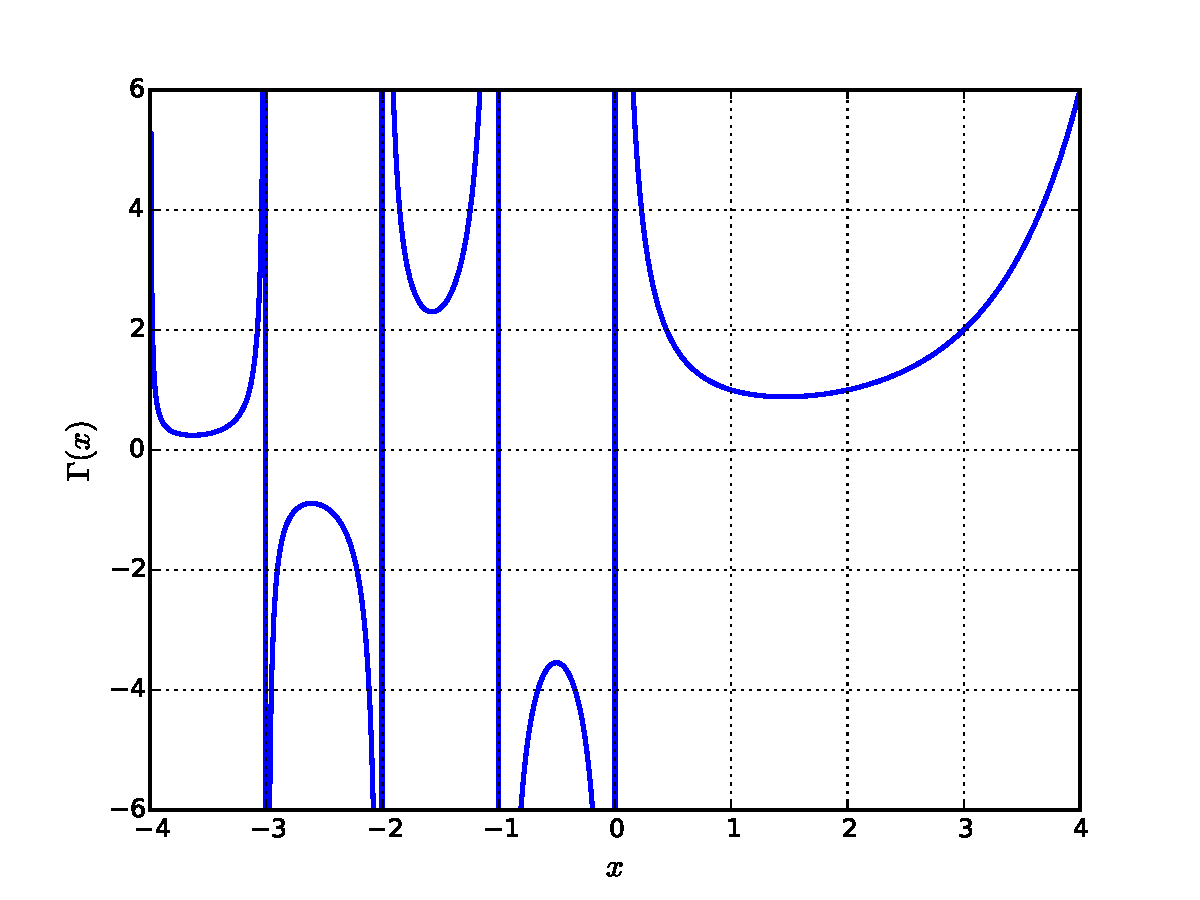
\includegraphics[angle=0,width=0.7\textwidth]{figs/fig-funcion-Gamma.pdf}
\caption{La funci'on $\Gamma$ con argumento real. C'odigo Python \href{https://github.com/gfrubi/FM2/blob/master/figuras-editables/fig-Gamma.py}{aqu\'i}.}
\label{fig-Gamma}
\end{figure}
